\documentclass[tikz,border=2pt]{standalone}
\usepackage{amsmath}
\usetikzlibrary{arrows.meta,decorations.pathreplacing}
\begin{document}
% Select table with select period r = 2: rows = age at selection, columns = duration 0, 1 and ultimate.
% A life selected at 40 uses q_[40] = 0.005, q_[40]+1 = 0.007, then ultimate q_42 = 0.01 (then q_43, ...),
% so 3p_[40] = 0.995(0.993)(0.99) = 0.97815465. Shaded cells share attained age 42 but are different rates.
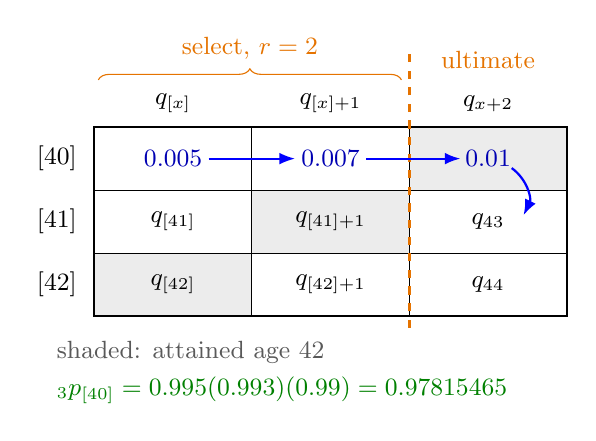
\begin{tikzpicture}[font=\small, >={Latex[length=2mm]}]
  \def\w{2.0} \def\h{0.8}
  % cells with attained age 42
  \fill[gray!15] (0,-3*\h) rectangle (\w,-2*\h);
  \fill[gray!15] (\w,-2*\h) rectangle (2*\w,-\h);
  \fill[gray!15] (2*\w,-\h) rectangle (3*\w,0);
  % grid
  \draw[thick] (0,-3*\h) rectangle (3*\w,0);
  \foreach \c in {1,2} \draw (\c*\w,-3*\h) -- (\c*\w,0);
  \foreach \r in {1,2} \draw (0,-\r*\h) -- (3*\w,-\r*\h);
  \draw[orange!90!black, very thick, dashed] (2*\w,-3*\h-0.15) -- (2*\w,0.95);
  % column headers
  \node at (0.5*\w,0.3) {$q_{[x]}$};
  \node at (1.5*\w,0.3) {$q_{[x]+1}$};
  \node at (2.5*\w,0.3) {$q_{x+2}$};
  \draw[orange!90!black, decorate, decoration={brace, amplitude=4pt}] (0.05,0.6) -- (2*\w-0.1,0.6)
    node[midway, above=4pt] {select, $r=2$};
  \node[orange!90!black, anchor=south] at (2.5*\w,0.62) {ultimate};
  % row labels
  \foreach \r/\a in {0/40,1/41,2/42} \node[anchor=east] at (-0.1,-\r*\h-0.5*\h) {$[\a]$};
  % entries
  \node[blue!70!black] at (0.5*\w,-0.5*\h) {$0.005$};
  \node[blue!70!black] at (1.5*\w,-0.5*\h) {$0.007$};
  \node[blue!70!black] at (2.5*\w,-0.5*\h) {$0.01$};
  \node at (0.5*\w,-1.5*\h) {$q_{[41]}$};
  \node at (1.5*\w,-1.5*\h) {$q_{[41]+1}$};
  \node at (2.5*\w,-1.5*\h) {$q_{43}$};
  \node at (0.5*\w,-2.5*\h) {$q_{[42]}$};
  \node at (1.5*\w,-2.5*\h) {$q_{[42]+1}$};
  \node at (2.5*\w,-2.5*\h) {$q_{44}$};
  % path of a life selected at 40
  \draw[blue, thick, ->] (0.5*\w+0.45,-0.5*\h) -- (1.5*\w-0.45,-0.5*\h);
  \draw[blue, thick, ->] (1.5*\w+0.45,-0.5*\h) -- (2.5*\w-0.35,-0.5*\h);
  \draw[blue, thick, ->] (2.5*\w+0.3,-0.65*\h) to[bend left=40] (2.5*\w+0.45,-1.4*\h);
  % notes
  \node[gray!70!black, anchor=north west] at (-0.6,-3*\h-0.2) {shaded: attained age $42$};
  \node[green!50!black, anchor=north west] at (-0.6,-3*\h-0.65) {${}_3p_{[40]}=0.995(0.993)(0.99)=0.97815465$};
\end{tikzpicture}
\end{document}
